\section{ainulfiliani (1174073)}
\subsection{LeafletJS dan MapProxy}
\begin{enumerate}
    \item Jalankan terlebih dahulu mapproxy pada folder gede dengan menggunakan setingan agm.yaml
        \hfill\break
        \begin{figure}[H]
        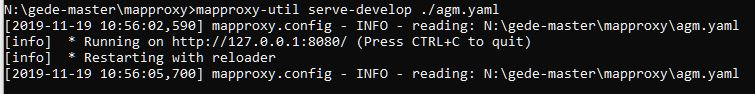
\includegraphics[width=4cm]{figures/tugas5/1174073/1.jpg}
        \centering
        \caption{Menjalankan Mapproxy}
        \end{figure}
        
        
    \item Setelah itu buka contoh file leafletjs yang ada di dalam folder gede  yang telah kita download sebelumnya .
    
  \hfill\break
  \begin{figure}[H]
  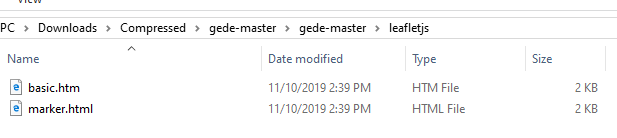
\includegraphics[width=4cm]{figures/tugas5/1174073/2.jpg}
  \centering
  \caption{Isi Basic.html}
  \end{figure}
  
    \item Setelah itu buka file basic.html pada folder leafletjs yang ada di dalam folder gede menggunakan browser
        \hfill\break
        \begin{figure}[H]
        
        
        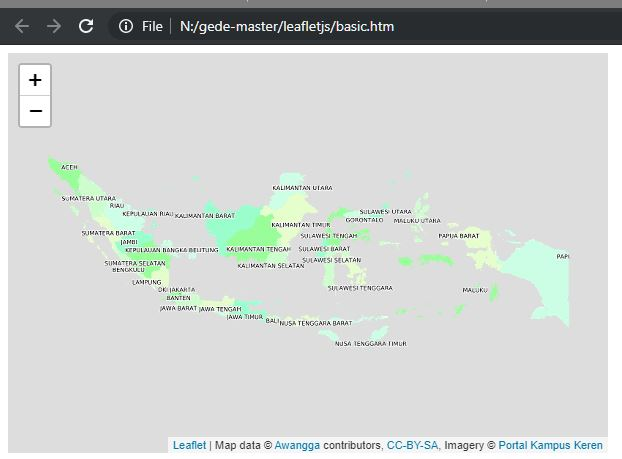
\includegraphics[width=4cm]{figures/tugas5/1174073/3.jpg}
        \centering
        \caption{Hasil dari file basic.htm}
        \end{figure}
   \item Dengan menggunakan LeafletJS kita dapat menambahkan marker, circle dan polygon yaitu dengan cara seperti gambar dibawah ini yang ada pada file marker.html pada folder gede/leafletjs
        \hfill\break
        \begin{figure}[H]
        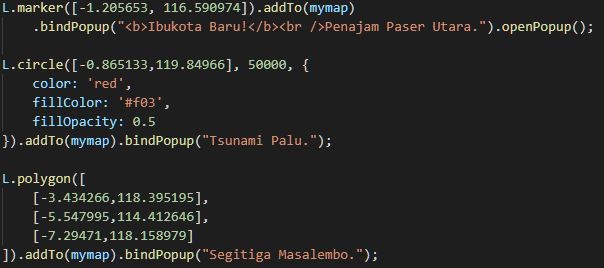
\includegraphics[width=4cm]{figures/tugas5/1174073/4.jpg}
        \centering
        \caption{Contoh menambahkan marker, circle dan polygon}
        \end{figure}
   \item Apabila file tersebut dibuka di browser maka akan muncul seperti ini
        \hfill\break
        \begin{figure}[H]
        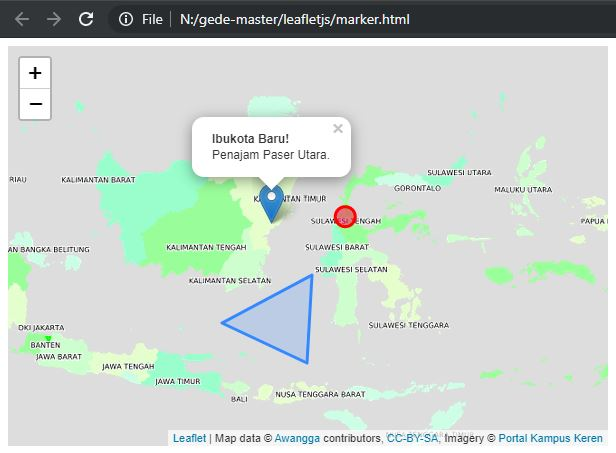
\includegraphics[width=4cm]{figures/tugas5/1174073/5.jpg}
        \centering
        \caption{Hasil dari file marker.html}
        \end{figure}
\end{enumerate}
\subsection{Link Youtube LeafletJS dan MapProxy}
https://youtu.be/iAg1eAVkTqY

